\documentclass[tikz]{standalone}
\usepackage{pgfplots}
\pgfplotsset{compat=1.15}
\usepackage{mathrsfs}
\usetikzlibrary{arrows,calc}
\usepackage{tkz-euclide}
\pagestyle{empty}

\definecolor{AngleClr}{rgb}{0,0.39215686274509803,0}
\definecolor{ShapeClr}{rgb}{0.6,0.2,0}
\definecolor{SquareClr}{RGB}{250, 248, 217}
\definecolor{GreenDist}{RGB}{7,122,7}
\definecolor{RedDist}{RGB}{232,57,14}

\definecolor{BlueSqr}{RGB}{5,81,163}
\definecolor{RedSqr}{RGB}{0, 156, 0}

\begin{document}

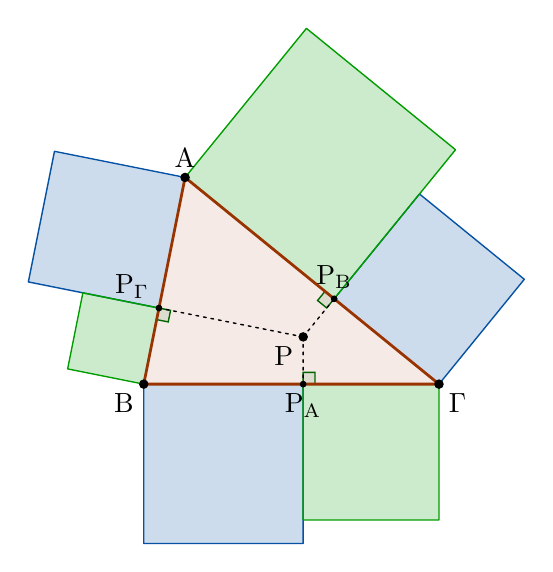
\begin{tikzpicture}[scale=.75]
\tkzSetUpLine[line width=1pt,color=black]
\tkzSetUpPoint[fill=black]

\tkzDefPoints{0/0/B,0.7/3.5/A,5/0/C,2.7/0.8/P}

\tkzDefPointBy[projection=onto B--C](P)\tkzGetPoint{PA}
\tkzDefPointBy[projection=onto A--C](P)\tkzGetPoint{PB}
\tkzDefPointBy[projection=onto A--B](P)\tkzGetPoint{PC}


\tkzFillPolygon[fill=ShapeClr,fill opacity=0.1](A,B,C)

\tkzMarkRightAngles[line width=0.5pt, size=.2,color=AngleClr,fill=AngleClr,fill opacity=0.1](P,PA,C P,PC,B P,PB,A)

\tkzDrawSegments[line width=0.5pt,color=black,dashed,dash pattern=on 1pt off 1.75pt](P,PA P,PB P,PC)

\tkzDefSquare(PC,A)
\tkzDrawPolygon[fill=BlueSqr,color=BlueSqr,fill opacity=0.2,line width=0.5pt](PC,A,tkzFirstPointResult, tkzSecondPointResult)
\tkzDefSquare(PA,B)
\tkzDrawPolygon[fill=BlueSqr,color=BlueSqr,fill opacity=0.2,line width=0.5pt](PA,B,tkzFirstPointResult, tkzSecondPointResult)
\tkzDefSquare(PB,C)
\tkzDrawPolygon[fill=BlueSqr,color=BlueSqr,fill opacity=0.2,line width=0.5pt](PB,C,tkzFirstPointResult, tkzSecondPointResult)


\tkzDefSquare(A,PB)
\tkzDrawPolygon[fill=BlueSqr,color=RedSqr,fill opacity=0.2,line width=0.5pt](A,PB,tkzFirstPointResult, tkzSecondPointResult)

\tkzDefSquare(B,PC)
\tkzDrawPolygon[fill=BlueSqr,color=RedSqr,fill opacity=0.2,line width=0.5pt](B,PC,tkzFirstPointResult, tkzSecondPointResult)

\tkzDefSquare(C,PA)
\tkzDrawPolygon[fill=BlueSqr,color=RedSqr,fill opacity=0.2,line width=0.5pt](C,PA,tkzFirstPointResult, tkzSecondPointResult)


\tkzDrawPolygon[color=ShapeClr](A,B,C)

\tkzDrawPoints[size=3](A,B,C,P)
\tkzDrawPoints[size=2](PA,PB,PC)

\tkzLabelPoint[above](A){$\rm A$}
\tkzLabelPoint[below left](B){$\rm B$}
\tkzLabelPoint[below right](C){$\rm \Gamma$}
\tkzLabelPoint[below left](P){$\rm P$}
\tkzLabelPoint[below](PA){$\rm P_A$}
\tkzLabelPoint[above](PB){$\rm P_B$}
\tkzLabelPoint[above left](PC){$\rm P_\Gamma$}

\end{tikzpicture}
\end{document}
